\chapter{付録}

\section{学習時のパラメータ}
\label{sec:appendix_params}

提案モデルの学習時のパラメータの値を表\ref{tab:params1}に示す。また、Adam~\cite{Adam}の疑似コード~(Algorithm~\ref{alg:Adam})~にあるハイパーパラメータの値を表\ref{tab:params2}に示す。

\begin{table}[b]
\begin{center}
\begin{minipage}{0.49\hsize}
    \begin{center}
        \begin{tabular}{lr}\toprule
            パラメータ & 値 \\ \midrule
            バッチサイズ & 1 \\ 
            エポック数 & 1000 \\ \bottomrule
        \end{tabular}
    \end{center}
    \caption{}
    \label{tab:params1}
\end{minipage}
\begin{minipage}{0.49\hsize}
    \begin{center}
        \begin{tabular}{lr}\toprule
            パラメータ & 値 \\ \midrule
            $\beta_1$ & 0.5 \\
            $\beta_2$ & 0.999 \\
            $\eta$ & 0.0002 \\ 
            $\epsilon$ & $10^{-8}$ \\ \bottomrule
        \end{tabular}
    \end{center}
    \caption{}
    \label{tab:params2}
\end{minipage}
\end{center}
\end{table}

\begin{algorithm}[b]
\label{alg:Adam}
    \DontPrintSemicolon
    %\SetAlgoNoEnd\SetAlgoNoLine
    \SetKwInOut{KwHyParam}{HyperParameter}
    \SetKwInOut{KwParam}{Parameter}
    \SetKwInOut{KwObFunc}{Objective~Function}
    \KwHyParam{$\beta_1,\beta_2\in \interval[open left]{0}{1},\eta,\epsilon$}
    \KwObFunc{$f$}
    \KwParam{$\theta$}
    \Init{
        \settowidth{\maxwidth}{$m_1,m_2 \leftarrow 0,0$~}
        \algalign{$t \leftarrow 0$~}{(Initialize~timestep)\;}
        \algalign{$\theta \leftarrow \theta_0$~}{(Initialize~Parameter)\;}
        \algalign{$m_1,m_2 \leftarrow 0,0$~}{(Initialize~moments)\;}
    }
    \Proc{
        \While{$\theta$ not converged}{
            \settowidth{\maxwidth}{$m_1,m_2 \leftarrow \beta_1 \cdot m_1+(1-\beta_1) \cdot g,\beta_2 \cdot m_2+(1-\beta_2) \cdot (g \odot g)$~}
            \algalign{$t \leftarrow t+1$~}{(Update~timestep)\;}
            \algalign{$g \leftarrow \nabla _{\theta} f(\theta)$~}{(Compute~gradient~of~$f(\theta)$)\;}
            \algalign{$m_1,m_2 \leftarrow \beta_1 \cdot m_1+(1-\beta_1) \cdot g,\beta_2 \cdot m_2+(1-\beta_2) \cdot (g \odot g)$~}{(Update~biased~moments)\;}
            \algalign{$\hat{m_1},\hat{m_2} \leftarrow m_1/(1-\beta_1^t),m_2/(1-\beta_2^t)$~}{(Update~bias-corrected~moments)\;}
            \algalign{$\theta \leftarrow \theta - \eta \cdot \hat{m_1}/(\sqrt{\hat{m_2}}+\epsilon)$~}{(Update~Parameter)\;}
        }
        \Return{$\theta$}\;
    }
\caption{Adam~\cite{Adam}の疑似コード}
\end{algorithm}

%ここで改ページ

\section{データセットの分割}
\label{sec:appendix_split}

22音ずつの4つのサブセットにデータセットを分割した~(図\ref{fig:data_div})~。また、データセットの4分割は、88音をシャッフルして配列に格納した後に22音ずつ順に選ぶことで実装した。

\begin{figure}[h]
\begin{center}
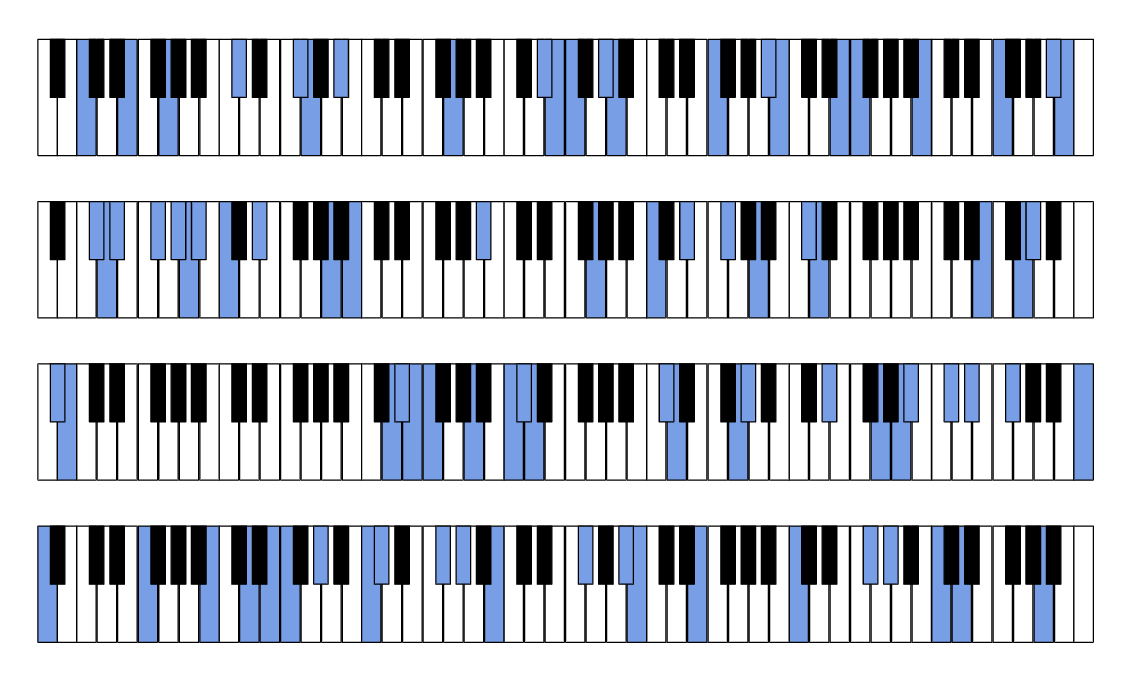
\includegraphics[width=\hsize]{figure/data_div.png}
\caption{データセットのサブセット}
\label{fig:data_div}
\end{center}
\end{figure}

\begin{comment}
\begin{table}[h]
\label{tab:split}
\caption{}
\begin{center}
    \scalebox{0.7}{
    \begin{tabular}{l|llllllllllllllllllllll}\toprule
        番号  \\ \midrule
        0 & C1 & E1 & G1 & C2$\sharp$ & F2$\sharp$ & G2 & A2$\sharp$ & G3 & D4$\sharp$ & E4 & F4 & G4$\sharp$ & A4 & F5 & A5$\sharp$ & B5 & E6 & F6 & B6 & F7 & A7$\sharp$ & B7\\ 
        1 & C1$\sharp$ & D1 & D1$\sharp$ & F1$\sharp$ & G1$\sharp$ & A1 & A1$\sharp$ & C2 & D2$\sharp$ & A2 & B2 & A3$\sharp$ & G4 & C5 & D5$\sharp$ & F5$\sharp$ & A5 & C6$\sharp$ & D6 & E7 & G7 & G7$\sharp$ \\ 
        2 & A0$\sharp$ & B0 & D3 & D3$\sharp$ & E3 & F3 & A3 & C4 & C4$\sharp$ & D4 & C5$\sharp$ & D5 & G5 & G5$\sharp$ & D6$\sharp$ & G6 & A6 & A6$\sharp$ & C7$\sharp$ & D7$\sharp$ & F7$\sharp$ & C8 \\ 
        3 & A0 & F1 & B1 & D2 & E2 & F2 & G2$\sharp$ & C3 & C3$\sharp$ & F3$\sharp$ & G3$\sharp$ & B3 & F4$\sharp$ & A4$\sharp$ & B4 & E5 & C6 & F6$\sharp$ & G6$\sharp$ & C7 & D7 & A7 \\ \bottomrule
    \end{tabular}
    }
\end{center}
\end{table}
\end{comment}